\appendix

\begin{frame}
  \frametitle{Appendix}
  \framesubtitle{Kripke Structure}

  A \textbf{Kripke Structure} is a variation of the transition system\
  used in model checking to represent behavior of a system.

  \begin{block}{A \textit{Go} Program as a \textbf{Kripke Structure}}
    \begin{columns}
      \begin{column}{0.49\textwidth}
        \centering
        \inputminted[
          firstline=1,
          fontsize=\scriptsize,
          framesep=4mm]
        {go}{go/fibonnaci.go}
      \end{column}
      \begin{column}{0.49\textwidth}
        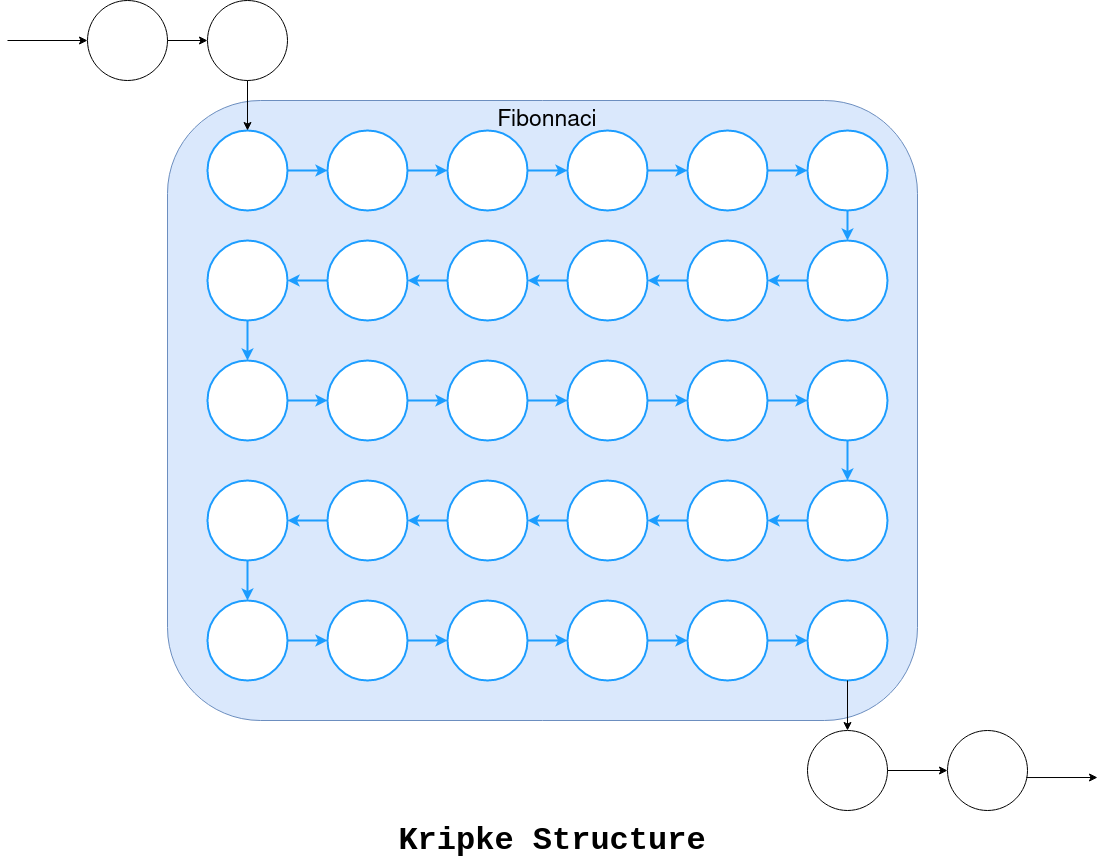
\includegraphics[width=6cm]{assets/FiboKripke.png}
      \end{column}
    \end{columns}
  \end{block}
\end{frame}

\begin{frame}
  \frametitle{Appendix}
  \framesubtitle{Recursive \texttt{struct}}

  \begin{block}{A \textit{Go} struct using another}
    \begin{columns}
      \begin{column}{0.49\textwidth}
        \centering
        This is not valid.
        \inputminted[
          firstline=3,
          lastline=9
          fontsize=\scriptsize,
          framesep=4mm]
        {go}{go/recursive.go}
      \end{column}
      \begin{column}{0.49\textwidth}
        \centering
        This is valid.
        \inputminted[
          firstline=3,
          lastline=9
          fontsize=\scriptsize,
          framesep=4mm]
        {go}{go/recursive2.go}
      \end{column}
    \end{columns}
  \end{block}
\end{frame}

\begin{frame}
  \frametitle{Appendix}
  \framesubtitle{Pointer receivers}

  \begin{block}{\textit{Go} pointer receivers}
    \centering
    \inputminted[
      firstline=3,
      fontsize=\scriptsize,
      framesep=4mm]
    {go}{go/pointerreceivers.go}
  \end{block}
\end{frame}

\begin{frame}
  \frametitle{Appendix}
  \framesubtitle{Interface}

  \begin{block}{\textit{Go} interface}
    \centering
    \inputminted[
      firstline=3,
      fontsize=\scriptsize,
      framesep=4mm]
    {go}{go/interface.go}
  \end{block}
\end{frame}
